\documentclass{report}
\usepackage{float}

% for the image in the title
\usepackage{tikz}

% custom spacing
\usepackage{setspace}
\onehalfspacing

% footer and header
\usepackage{fancyhdr}
% \setlength{\headheight}{15.2pt}

% underlining
\usepackage{ulem}


% Table of contents link to corresponding sections
\usepackage{hyperref}
\hypersetup{
	colorlinks,
	citecolor=black,
	filecolor=black,
	linkcolor=black,
	urlcolor=black
}

\usepackage{amsmath}
% Remove che "Chapter" string before chapters
\iffalse
\makeatletter
\def\@makechapterhead#1{%
	\vspace*{50\p@}%
	{\parindent \z@ \raggedright \normalfont
		\interlinepenalty\@M
		\Huge\bfseries  \thechapter.\quad #1\par\nobreak
		\vskip 40\p@
}}
\makeatother
\fi

% Fancy chapters
\usepackage[Bjarne]{fncychap}
% options: Sonny, Lenny, Glenn, Conny, Rejne, Bjarne, Bjornstrup

\begin{document}
	
	
	%title page
	\begin{titlepage}
		\begin{figure}[t]
			\centering
\includegraphics[width=0.3\textwidth]{images/unitn-logo}
		\end{figure}
		\begin{center}
			\textsc{ \LARGE{Università degli Studi di Trento \\}}
			\textsc{ \LARGE{Facoltà di Informatica\\ }}
			\textnormal{ \LARGE{Corso di Ingegneria del Software\\}}
			\vspace{30mm}
			\fontsize{10mm}{7mm}\selectfont 
			\textup{Fix Mi \\ Documento di Architettura}\\
		\end{center}
		
		\vspace{25mm}
		
		\centering
		\large Gruppo G43: \\ Giovanni Santini\\ Riginel Ungureanu \\ Valerio Asaro
		
		\vspace{20mm}
		
		\centering{\large{Anno Accademico 2023/2024 \\ Trento }}
		
	\end{titlepage}
	
	
	
	
	% use header and footers
	\pagestyle{fancy}
	\fancyhead[R]{\chaptername\ \thechapter}  % header
	
	%\maketitle
	\tableofcontents
	\newpage
	
	
	
	\section{Scopo del documento}
	
	
	
	
	\section{Informazioni del Documento}
	
	% table
	\begin{center} % center the table
		\centering
		\begin{tabular}{ |p{4cm}|p{4cm}|  }
			\hline
			\centering Campo & \qquad\qquad Valore \\ % I found no other way...
			\hline
			Titolo del Documento & Documento di Architettura \\
			\hline
			Titolo del Progetto & Fix Mi \\
			\hline
			Autori del Documento &
			Giovanni Santini \\ & Riginel Ungureanu \\ & Valerio Asaro \\
			\hline
			Amministratore Progetto & Riginel Ungureanu\\
			\hline
			Versione del documento & 1.0 \\
			\hline
		\end{tabular}
	\end{center}
	


\iffalse
\section{Nome}
\begin{figure}[H]
	\centering\includegraphics[width=1.2\textwidth]{URL}
	Nome dell'immagine
\end{figure}
\subsection*{Descrizione}
Descrivi generalmente cosa fa l'immagine mostrata

Per ogni classe fai una
\subsubsection{Nome}

in cui spieghi la classe dal punto di vista dell'alto livello, e i metodi (solo quelli non ovvi) mostrati.
In seguito descrivi come interagisce la classe analizzata con le altre.


\fi
	
\chapter{Diagramma delle Classi}

\section{Task}

\begin{figure}[H]
	\centering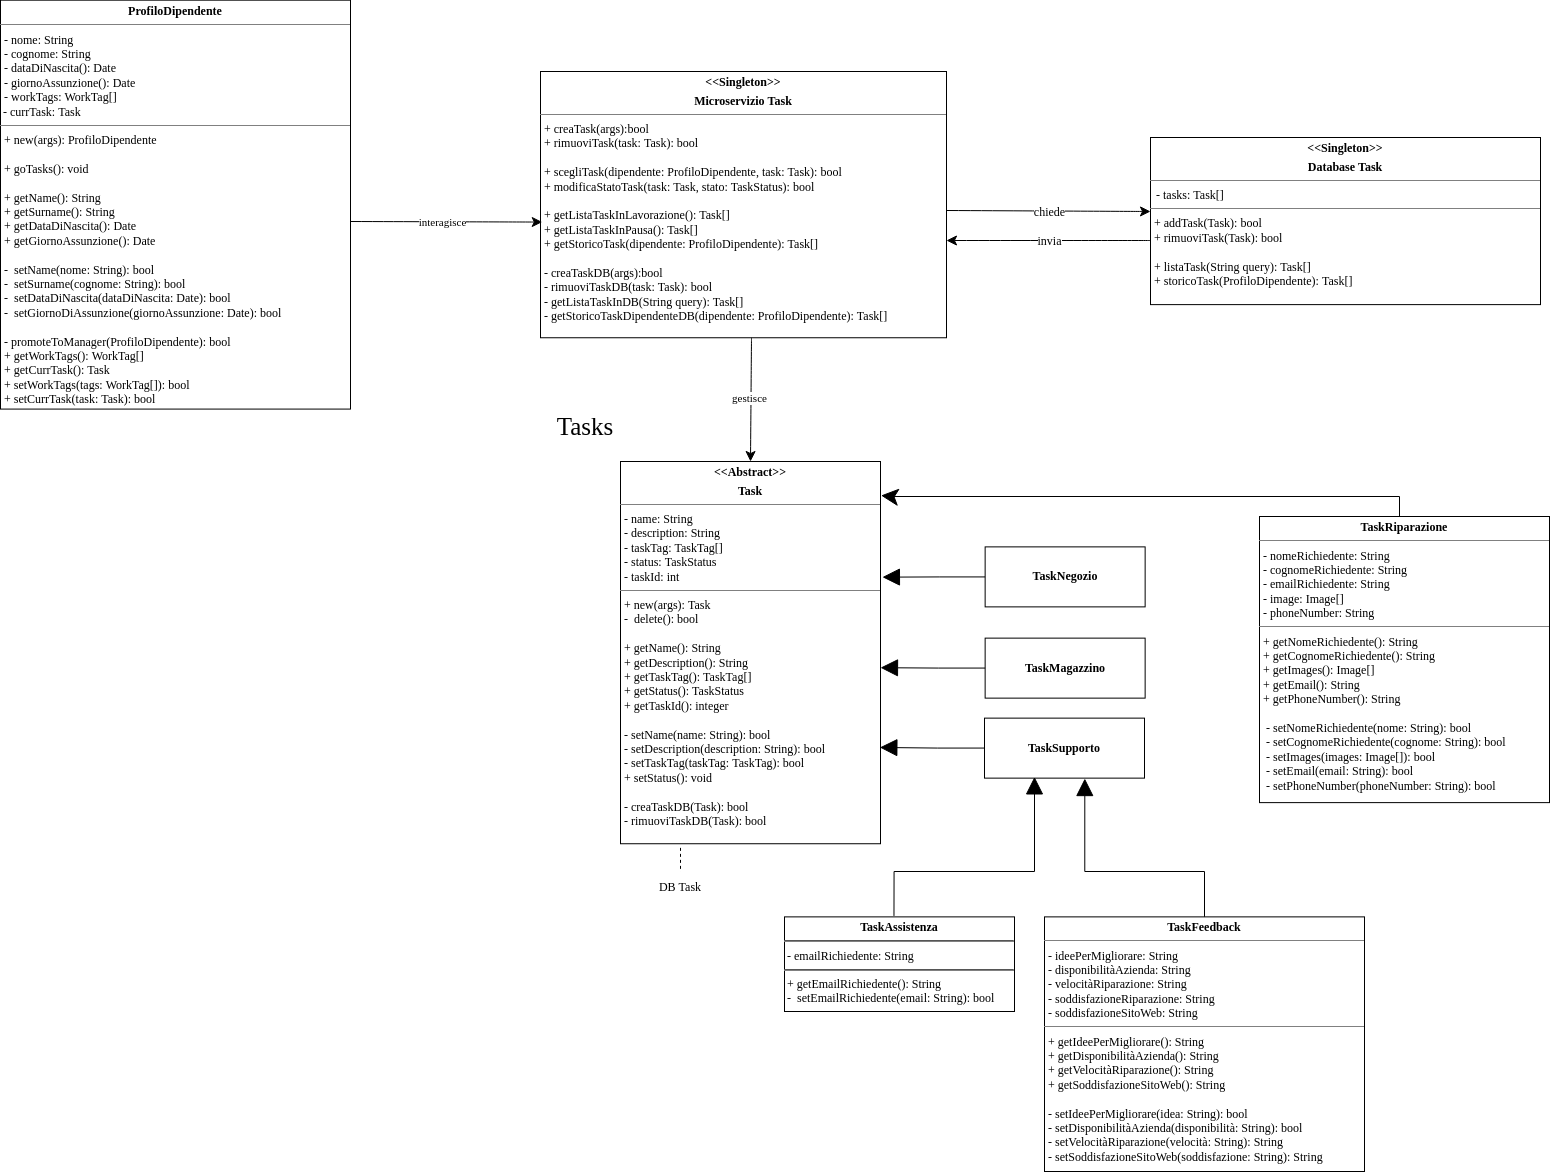
\includegraphics[width=1\textwidth]{images/Diagramma_delle_classi_task.png}
	Diagramma delle classi per la componente "Task"
\end{figure}
Data la componente "Task", seguendo ciò che è stato descritto nel Requisito Funzionale numero "9" e definita precedentemente nel rispettivo diagramma, sono state individuate le classi e relativi metodi e attributi di cui sotto:

\begin{figure}[H]
	\centering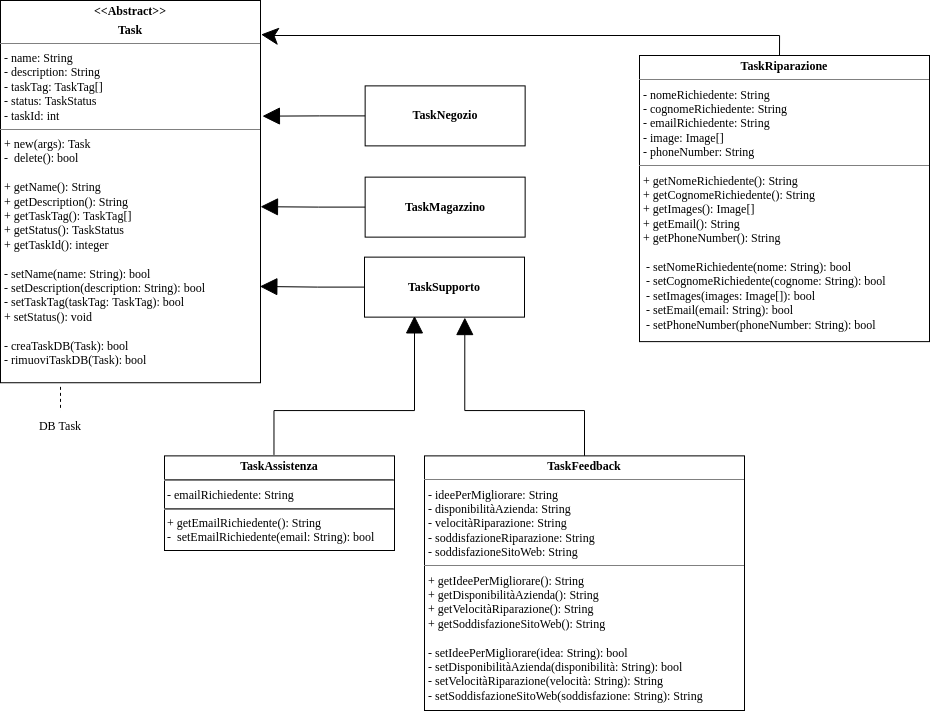
\includegraphics[width=1.2\textwidth]{images/Diagramma_delle_classi_task1.png}
	Diagramma delle classi per la componente "Task", 1
\end{figure}
\subsection*{Descrizione}
La classe "Task" definisce, come descritto dal Requisito Funzionale numero "9.1", l'oggetto "Task", da cui "TaskNegozio", "TaskMagazzino" e "TaskSupport" ereditano le proprietà. Le variabili di tipo "Task" vengono poi utilizzate dalla classe "Microservizio Task".

%Aggiungere Analisi di ogni classe

\begin{figure}[H]
	\centering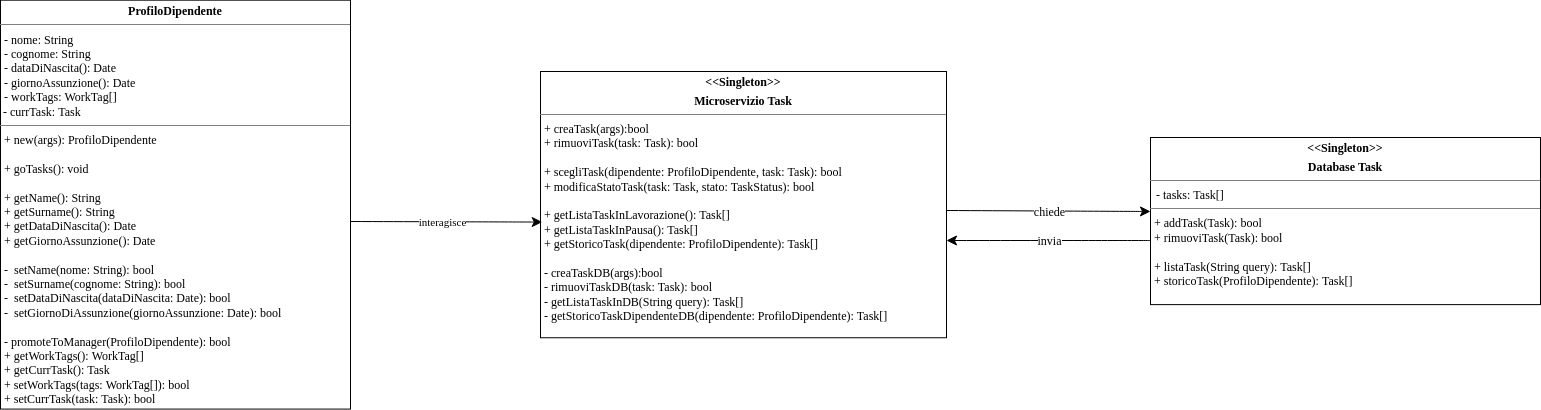
\includegraphics[width=1.2\textwidth]{images/Diagramma_delle_classi_task2.png}
	Diagramma delle classi per la componente "Task", 2
\end{figure}
\subsection*{Descrizione}
La classe "Microservizio Task" permette al dipendente di interagire con le tasks disponibili all'interno del sistema. In particolare potrà visualizzare le tasks in esecuzione ed aggiornare lo stato di una task, interagendo con il DataBase Task, come definito dal Requisito Funzionale numero "9.3". Per tale fine, osservando il diagramma di contesto e delle componenti definiti precedentemente, sono state individuate le seguenti classi: 

\subsubsection*{Microservizio Task}
Si pone come tramite tra il dipendente ed il Database Task. Invia e riceve informazioni riguardanti le Task dal Database, permette al dipendente di creare una task, rimuoverla o sceglierla (Cambiandone lo stato in "In Lavorazione"). Per tale scopo, sono stati individuati i seguenti metodi ed attributi:

\begin{itemize}
\item task: Task[]
\begin{itemize}
    \item L'insieme di oggetti "Task" memorizzato in maniera persistente.
\end{itemize}
\item public creaTask(args):bool
\begin{itemize}
    \item Crea un nuovo oggetto di tipo "Task", ritorna un valore booleano per indicare il successo dell'operazione. Gli argomenti contengono i valori dei campi appartenenti alla classe "Task". 
\end{itemize}
\item public rimuoviTask(task: Task): bool
\begin{itemize}
    \item Rimuove un oggetto di tipo "Task", ritorna un valore booleano per indicare il successo dell'operazione. L'argomento è l'oggetto "Task" da eliminare.
\end{itemize}
\item public scegliTask(dipendente: ProfiloDipendente, task: Task): bool
\begin{itemize}
    \item Sceglie un oggetto di tipo "Task" da assegnare ad un dipendente, fallisce nel caso in cui un dipendente stia ancora lavorando ad un altra task.
\end{itemize}
\item public modificaStatoTask(task: Task, stato: TaskStatus): bool
\begin{itemize}
    \item Modifica lo stato di un oggetto di tipo "Task", ritorna un valore booleano per indicare il successo dell'operazione.
\end{itemize}
\item public getListaTaskInLavorazione(): Task[]
\begin{itemize}
    \item Ritorna una lista di tipo "Task" contenente oggetti "Task" che sono ancora "In Lavorazione".
\end{itemize}
\item public getListaTaskInPausa(): Task[]
\begin{itemize}
    \item Ritorna una lista di tipo "Task" contenente oggetti "Task" che sono "In Pausa".
\end{itemize}
\item public getStoricoTask(dipendente: ProfiloDipendente): Task[]
\begin{itemize}
    \item Ritorna una lista di tipo "Task" contenente oggetti "Task" completati da un dato dipendente.
\end{itemize}
\item private creaTaskDB(args):bool
\begin{itemize}
    \item Salva i dati di un oggetto di tipo "Task" all'interno del Database, ritorna un valore booleano per indicare il successo dell'operazione.
\end{itemize}
\item private rimuoviTaskDB(task: Task): bool
\begin{itemize}
    \item Rimuove i dati di un oggetto di tipo "Task" dal Database, ritorna un valore booleano per indicare il successo dell'operazione.
\end{itemize}
\item private getListaTaskInDB(String query): Task[]
\begin{itemize}
    \item Ritorna una lista di tipo "Task" contenente il risultato  di una richiesta effettuata sul Database.
\end{itemize}
\item private getStoricoTaskDipendenteDB(dipendente: ProfiloDipendente): Task[]
\begin{itemize}
    \item Ritorna una lista di tipo "Task" contenente lo storico delle task svolte da un dipendente, effettuando una richiesta al DataBase.
\end{itemize}
\end{itemize}

\subsubsection*{Database Task}
La classe "Database Task" permette al Microservizio Task di interfacciarsi con il Database, fornisce metodi utili alla memorizzazione delle tasks, alla loro gestione ed al loro recupero. I metodi individuati sono i seguenti:
\begin{itemize}
\item public addTask(Task): bool
\begin{itemize}
    \item Aggiunge un nuovo elemento di tipo "Task" al Database, ritorna un valore booleano per indicare il successo dell'operazione.
\end{itemize}
\item public rimuoviTask(Task): bool
\begin{itemize}
    \item Rimuove un elemento esistente di tipo "Task" dal Database, ritorna un valore booleano per indicare il successo dell'operazione.
\end{itemize}
\item public listaTask(String query): Task[]
\begin{itemize}
    \item Ritorna una lista di tipo "Task", risultato della ricerca fatta all'interno del Database tramite la stringa "query".
\end{itemize}
\item public storicoTask(ProfiloDipendente): Task[]
\begin{itemize}
    \item Ritorna una lista di tipo "Task" contenente tutte le task completate dal profilo dipendente richiesto.
\end{itemize}
\end{itemize}

\subsubsection*{Profilo Dipendente}
Il dipendente può accedere alla pagina "Tasks"( in cui le può visualizzare, gestire, creare ed eliminare) attraverso il seguente metodo:

\begin{itemize}
\item public goTasks(): void
\begin{itemize}
    \item Porta il dipendente nella pagina per gestire le tasks.
\end{itemize}
\iffalse
METODI PER IL PROFILO
\item public new(args): ProfiloDipendente
\begin{itemize}
    \item Crea e restituisce un nuovo profilo dipendente passando tutte le informazioni necessarie quali "nome", "cognome", "data di nascita" e "giorno di assunzione" come argomenti.
\end{itemize}
\item public getName(): String
\begin{itemize}
    \item Ritorna il nome del profilo dipendente.
\end{itemize}
\item public getSurname(): String
\begin{itemize}
    \item Ritorna il cognome del profilo dipendente.
\end{itemize}
\item public getDataDiNascita(): Date
\begin{itemize}
    \item Ritorna il giorno di nascita del profilo dipendente.
\end{itemize}
\item public getGiornoAssunzione(): Date
\begin{itemize}
    \item Ritorna il giorno di assunzione del profilo dipendente.
\end{itemize}
\item private setName(nome: String): bool
\begin{itemize}
    \item Imposta il nome del profilo dipendente, ritorna un valore booleano per indicare il successo dell'operazione.
\end{itemize}
\item private setSurname(cognome: String): bool
\begin{itemize}
    \item Imposta il cognome del profilo dipendente, ritorna un valore booleano per indicare il successo dell'operazione.
\end{itemize}
\item private  setDataDiNascita(dataDiNascita: Date): bool
\begin{itemize}
    \item Imposta la data di nascita del profilo dipendente, ritorna un valore booleano per indicare il successo dell'operazione.
\end{itemize}
\item private setGiornoDiAssunzione(giornoAssunzione: Date): bool
\begin{itemize}
    \item Imposta il giorno di assunzione del profilo dipendente, ritorna un valore booleano per indicare il successo dell'operazione.
\end{itemize}
\item private promoteToManager(ProfiloDipendente): bool
\begin{itemize}
    \item Trasforma un profilo dipendente in un profilo manager, ritorna un valore boolean per indicare il successo dell'operazione.
\end{itemize}
FINE METODI PER IL PROFILO
\fi
\iffalse
METODI NON CERTI
\item public getWorkTags(): WorkTag[]
\begin{itemize}
    \item Riceve le Work Tags del profilo dipendente.
\end{itemize}
\item public getCurrTask(): Task
\begin{itemize}
    \item Ritorna un oggetto di tipo "Task", che rappresenta la task a cui il dipendente sta lavorando in quel momento.
\end{itemize}
\item public setWorkTags(tags: WorkTag[]): bool
\begin{itemize}
    \item Imposta le Work Tags del profilo dipendente, ritorna un valore booleano per indicare il successo dell'operazione.
\end{itemize}
\item public setCurrTask(task: Task): bool
\begin{itemize}
    \item Imposta un oggetto di tipo "Task" come task a cui il dipendente sta lavorando in quel momento, ritorna un valore booleano per indicare il successo dell'operazione.
\end{itemize}
FINE METODI NON CERTI
\fi
\end{itemize}











\chapter{Codice in Object Constraint Language}	
	
\chapter{Diagramma delle classi con codice OCL}
	
\end{document}